\documentclass[10pt,letterpaper,addpoints]{exam}
\usepackage[utf8]{inputenc}
\usepackage[spanish,es-noshorthands]{babel}
\usepackage{hyperref}
\usepackage{amsmath}
\usepackage{amsfonts}
\usepackage{amssymb}
\usepackage{graphicx}
\usepackage{multicol}
\usepackage{tikz,pgf}
\usepackage[left=2cm,right=2cm,top=2cm,bottom=2cm]{geometry}
%\printanswers
\begin{document}
\title{\begin{minipage}{.2\textwidth}
        
\includegraphics[height=1.75cm]{Images/logo-colegio.png}
       \end{minipage}
\begin{minipage}{.55\textwidth}
 \begin{center}
 Prueba Bimestral I\\Matemáticas 11$^{\circ}$
\end{center}
\end{minipage}
\begin{minipage}{.2\textwidth}

\includegraphics[height=1.75cm]{Images/logo-sed.png} 
\end{minipage}
}
\author{Germ\'{a}n Avendaño Ram\'{i}rez~\thanks{Lic. Mat. U.D., M.Sc. U.N.}}
\date{}
\maketitle
\begin{center}
\fbox{\fbox{\parbox{5.5in}{\centering
\emph{\textbf{Formulario A}}. Conteste las preguntas en el cuadro de respuesta diseñado para tal fin}}}
\end{center}
\vspace{0.1in}
\begin{multicols}{2}
\begin{questions}
\question
Si en la expresión $ x^2y $, el valor de $ x $ se disminuye en un 40\% y el valor de $ y $ en un 25\%, entonces el valor de la expresión disminuye en un

\begin{oneparchoices}
\CorrectChoice 73\% \choice 32,5\% \choice 27\% \choice 22,5\%
\end{oneparchoices}
\question
De dos varillas cuyas longitudes son 360 cm y 108 cm, respectivamente, se desea obtener trozos iguales que tengan la longitud máxima posible. El mayor número total de trozos obtenidos es

\begin{oneparchoices}
\CorrectChoice 13 \choice 12 \choice 18 \choice 16     
\end{oneparchoices}
\question Si se trasladan los cuatro puntos 5 unidades a la izquierda y 2 unidades hacia arriba, las coordenadas de los nuevos puntos serán, respectivamente
\begin{center}
    \begin{tikzpicture}[scale=.5]
\draw[->] (-.5,0) -- (11.5,0);
\draw[->] (0,-.5) -- (0,8.5);
\node[below] (x) at (11.2,0) {$x$};
\node[left] (y) at (0,8.2) {$y$};
\fill (1,1)node[left]{A(1,1)} circle (.5ex);
\fill (11,3) node[left]{B(11,3)}circle (.5ex) ;
\fill (10,8) node[left]{C(10,8)} circle (.5ex);
\fill (0,6) node[left]{D(0,6)} circle (.5ex);
\end{tikzpicture} 
\end{center}
\begin{choices}
  \CorrectChoice $(-4,3), (6,5), (5,10), (-5,8)$
  \choice $(6,-1), (16,1), (15,6), (5,4)$
  \choice $(-4,-1), (6,1), (5,6), (-5,4)$
  \choice $(6,3), (16,5), (15,6), (-5,4)$
\end{choices}
  \question La gráfica que representa correctamente el subconjunto \[ S=\{(x,y)/ -1\leq x\leq 1, \quad 0\leq y \leq x+1\} \text{ es} \]
\begin{choices}
\begin{multicols}{2}
\CorrectChoice 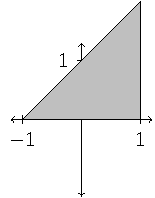
\includegraphics[scale=.75]{Images/desigA.pdf} 
\choice 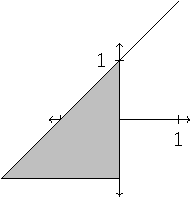
\includegraphics[scale=.75]{Images/desigB.pdf} 
\choice 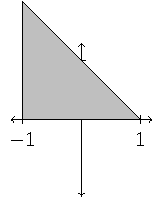
\includegraphics[scale=.75]{Images/desigC.pdf} 
\choice 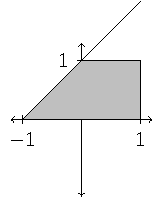
\includegraphics[scale=.75]{Images/desigD.pdf} 
\end{multicols}
\end{choices}
\question Un cono circular recto de volumen $C$, un cilindro de volumen $D$ y una esfera de volumen $E$ tienen todos, el mismo radio; el cono y el cilindro tiene la misma altura y ésta es igual al diámetro de la esfera. De acuerdo con la información anterior es correcto afirmar que
\begin{choices}
  \choice $ 2C+2D=3E $
  \choice $ C+D=E $
  \choice $ 2C=D+E $
  \CorrectChoice $ C-D+E=0 $
\end{choices}
\uplevel{Conteste \ref{firstq}--\ref{lastq}. En la siguiente recta numérica, se han señalado algunos puntos con sus respectivas coordenadas.}
 \begin{center}
  \begin{tikzpicture}[scale=5,>=stealth]
\draw[<->] (-1.2,0) -- (0.30,0);
\draw[thick] (-1,-.03) node[below]{$-1$}-- (-1,.03)node[above]{A};
\draw[thick] (-0.25,-.03) node[below]{$-\frac{1}{4}$}-- (-.25,.03)node[above]{B};
\draw[thick] (-.125,-.03) node[below]{$-\frac{1}{8}$}-- (-.125,.03)node[above]{C};
\draw[thick] (0,-.03) node[below]{$0$}-- (0,.03)node[above]{D};
\draw[thick] (.125,-.03) node[below]{$\frac{1}{8}$}-- (.125,.03)node[above]{E};
\draw[thick] (.25,-.03) node[below]{$\frac{1}{4}$}-- (.25,.03)node[above]{F};
\end{tikzpicture}
\end{center}
\question \label{firstq}Si $\overline{DE}$ se divide en $n$ segmentos congruentes (de igual medida), la longitud de cada uno de los $n$ segmentos es:
\begin{choices}
\begin{multicols}{2}
\choice $\dfrac{1}{n}$
\choice $\dfrac{4}{n}$
\CorrectChoice $\dfrac{1}{8n}$
\choice $\dfrac{8}{n}$
\end{multicols}
\end{choices}
\question Si $M$ y $N$ son los puntos medios de $\overline{AB}$ y $\overline{CD}$ respectivamente, la longitud de $\overline{MN}$ es,
\begin{choices}
\begin{multicols}{2}
 \choice $\dfrac{1}{2}$
 \choice $\dfrac{5}{8}$
 \choice $\dfrac{9}{16}$
 \CorrectChoice $\dfrac{11}{16}$
\end{multicols}
\end{choices}
\question \label{lastq} De la expresión $\left[\dfrac{1-\sqrt{3}}{2}\right]^{2}$, se puede afirmar que corresponde a un número
\begin{choices}
 \choice racional y se ubica en $\overline{AB}$
 \choice racional y se ubica en $\overline{BD}$
 \choice irracional y se ubica en $\overline{CD}$
 \CorrectChoice irracional y se ubica en $\overline{DE}$
\end{choices}
\question Al efectuar la operación $\dfrac{2}{3}-\dfrac{3}{4}$ se obtiene:

\begin{oneparchoices}
\choice $\dfrac{1}{4}$
\choice $-\dfrac{1}{7}$
\CorrectChoice $-\dfrac{1}{12}$
\choice $\dfrac{1}{12}$
\end{oneparchoices}
\question ¿Cuál de los siguientes intervalos corresponde a la solución de la inecuación $-5<x\leq 10$
\begin{choices}
\begin{multicols}{2}
\choice $[-5,10)$ 
\choice $(-5,10)$
\CorrectChoice $(-5,10]$
\choice $[-5,10]$
\end{multicols}
\end{choices}
\uplevel{Dados los conjuntos $A=(-2,8)$ y $B=(-\infty,\pi]$, responda las preguntas \ref{firstq1}--\ref{lastq1}}
\question \label{firstq1} El conjunto $A\cup B$ será el intervalo
\begin{choices}
\begin{multicols}{2}
 \choice $(-2,\pi)$
 \CorrectChoice $(-\infty,8)$
 \choice $(8,\pi]$
 \choice $(-\infty,\pi)$
\end{multicols}
\end{choices}
\question El conjunto $A \cap B $ será el intervalo
\begin{choices}
\begin{multicols}{2}
 \choice $(-2,\pi)$
 \CorrectChoice $(-2,\pi]$
 \choice $(-2,8)$
 \choice $[-2,8]$
\end{multicols}
\end{choices}
\question \label{lastq1} El complemento de $A$, que se simboliza $A^{c}$ y está conformado por los elementos que NO están en $A$ es:

\begin{choices}
 \choice $(-\infty,+\infty)$
 \CorrectChoice $(-\infty,-2]\cup [8,+\infty)$
 \choice $(-\infty,2)\cup (8,+\infty)$
 \choice $(-2,\pi]$
\end{choices}
\question Al solucionar la inecuación $3x\leq 18$ se obtiene
\begin{choices}
\begin{multicols}{2}
 \choice $(-\infty,6)$
 \CorrectChoice $(-\infty,6]$
 \choice $(6,+\infty)$
 \choice $[6,+\infty)$
\end{multicols}
\end{choices}
\begin{uplevel}{
 Una tabla de distribución de frecuencias con intervalos sirve para resumir un conjunto de datos estadísticos. Por ejemplo, ésta tabla muestra las 500 notas o calificaciones recibidas en el examen final del programa de ingeniería en una universidad.
\begin{center}
\begin{tabular}{|c|c|c|}\hline
Invervalo & Marca de clase & Frecuencia\\ \hline
[0,1) & 0.5 & 20\\ \hline
[1,2) & 1.5 & 21\\ \hline
[2,3) & 2.5 & 46\\ \hline
[3,4) & 3.4 & 283\\ \hline
[4,5) & 4.5 & 130\\ \hline
 \end{tabular}
 \end{center}
 La primera columna es la lista de los cinco intervalos en que se han agrupado las notas. La segunda, el punto medio de cada intervalo. La tercera muestra el número de notas de cada intervalo, es decir su frecuencia. (Por ejemplo hay 20 notas entre 0 y 1)
 
 Con base en esto, escoja la respuesta correcta en cada caso en las preguntas \ref{firstq2}--\ref{lastq2}.}
\end{uplevel}
\question \label{firstq2} La marca de clase es un número
\begin{choices}
\begin{multicols}{2}
 \choice Natural
 \choice entero
 \CorrectChoice Racional
 \choice Irracional
\end{multicols}
\end{choices}
\question ¿Cuántos estudiantes obtuvieron una nota menor que 1?

\begin{oneparchoices}
\CorrectChoice 20
\choice 21
\choice 46
\choice 130
\end{oneparchoices}
\question Si para aprobar el examen es necesario obtener una nota de 3 o más, ¿cuántos estudiantes aprobaron el examen?

\begin{oneparchoices}
 \choice 87
 \choice 283
 \CorrectChoice 413
 \choice 130
\end{oneparchoices}
\question Si un estudiante obtiene una nota de 4, pertenece al invervalo

\begin{oneparchoices}
 \choice [1,2) 
 \choice [2,3)
 \choice [3,4)
 \CorrectChoice [4,5)
\end{oneparchoices}
\question \label{lastq2} Al obtener una nota de 3, lo ubicamos en el intervalo

\begin{oneparchoices}
 \choice [1,2)
 \choice [2,3)
 \CorrectChoice [3,4)
 \choice [4,5)
\end{oneparchoices}
\begin{uplevel}{Conteste \ref{firstq4} con base en:
\begin{enumerate}
 \item[I] Si $x$ es un número real y $x<0$, entonces $\dfrac{1}{x}<0$
 \item[II] Si $x$ es un número entero, entonces $x$ es un número racional.
 \item[III] El producto de dos números primos es un número primo.
 \item[IV] Si $x$ es un número real, $\sqrt{x^{2}}=x$
\end{enumerate}
 }
\end{uplevel}
\question \label{firstq4} Es o son verdaderas

\begin{choices}
 \CorrectChoice I y II
 \choice III y IV
 \choice Solamente II
 \choice Solamente IV
\end{choices}
\question Un entero $n$ se denomina un número perfecto si es igual a la suma de todos sus divisores propios. 1 se cuenta como un divisor propio pero el número no. De los siguientes números el que NO es perfecto es

\begin{oneparchoices}
\choice 28
\choice 496
\CorrectChoice 2026
\choice 6
\end{oneparchoices}
\question Un profesor asigna 3 ejercicios. Pide a $\frac{1}{4}$ del número de estudiantes que está en clase que resuelvan el primer ejercicio, a $\frac{3}{8}$ que resuelvan el segundo, y a $\frac{5}{16}$ que resuelvan el tercero. Del total de alumnos dos están ausentes. La cantidad total de alumnos es:

\begin{oneparchoices}
 \choice 28
 \CorrectChoice 32
 \choice 38
 \choice 42
\end{oneparchoices}
\question Si la distancia entre dos puntos A y B de una recta numérica no es menor que 3, la gráfica que representa dos puntos con esta condición es:

\begin{choices}
\CorrectChoice 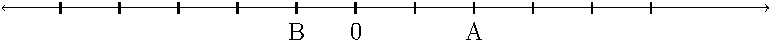
\includegraphics[scale=.5]{Images/respA.pdf} 
\choice 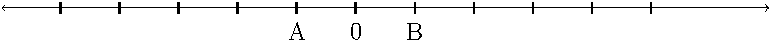
\includegraphics[scale=.5]{Images/respB.pdf} 
\choice 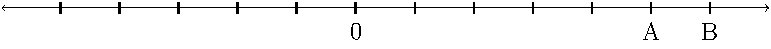
\includegraphics[scale=.5]{Images/respC.pdf} 
\choice 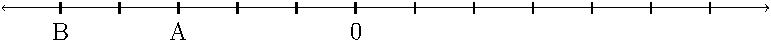
\includegraphics[scale=.5]{Images/respD.pdf} 
  \end{choices}
  \question
  La negación correcta de la proposición $P:$ Todos los números reales son racionales es:
  \begin{choices}
  \choice $\neg P$: Todos los números reales no son racionales
  \choice $\neg P$: Todos los números reales son irracionales
  \CorrectChoice $\neg P$: Algunos números reales son racionales
  \choice $\neg P$: Algunos números reales son no son números complejos 
\end{choices}  
\question Al hacer la tabla de verdad con las proposiciones $p$, $q$, $r$, $s$ y $t$ se deben considerar
\begin{choices}
\choice 10 posibilidades porque $2\times 5=10$
\choice 25 posibilidades porque $5^{2}=25$
\choice 10 posibilidades porque $2^{5}=10$
\CorrectChoice 32 posibilidades porque $2^{5}=32$
\end{choices}
\question Haga la tabla de verdad de la proposición compuesta 
\[[\neg(p\wedge q)]\Longleftrightarrow [\neg p \vee \neg q]\]
al respaldo de su cuadro de respuestas.
\fullwidth{\large Probabilidad}
\question En una caja blanca hay 3 fichas marcadas con los números 1, 2 y 3 respectivamente. En una caja negra hay 5 fichas marcadas con los números 1, 2, 3, 4 y 5 respectivamente. ¿Cuál de los siguientes diagramas de árbol representa los posibles resultados de sacar, al
azar, primero una ficha de la caja blanca y después una ficha de la caja negra?
\uplevel{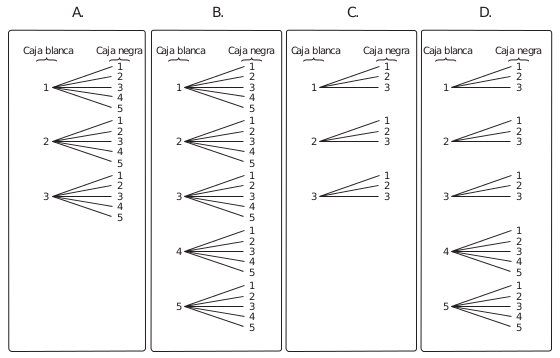
\includegraphics[scale=.46]{Images/diag-arbol.png}}
\question La siguiente tabla muestra, para tres años consecutivos, el valor del auxilio de transporte mensual que reciben los trabajadores de una empresa y el promedio de la tarifa de un pasaje para el servicio de transporte urbano en la ciudad:
\begin{center}
\begin{tabular}{|c|c|c|}
\hline 
\textbf{Año} & \textbf{Auxilio de transporte} & \textbf{Tarifa de un pasaje} \\ 
 & (mensual) & (promedio) \\ 
\hline 
2009 & \$59\,300 & \$1\,500 \\ 
\hline 
2010 & \$61\,500 & \$1\,600 \\ 
\hline 
2011 & \$63\,800 & \$1\,700 \\ 
\hline 
\end{tabular} 
\end{center}
Si un trabajador debe comprar al mes 40 pasajes, se puede afirmar que, con respecto al primer año, en el tercero el desequilibrio (el costo de transporte que no le cubre el auxilio) es
\begin{choices}
\begin{multicols}{2}
\choice Mayor en \$200
\choice Menor en \$4300
\choice 3 veces mayor
\CorrectChoice 6 veces mayor
\end{multicols}
\end{choices}
%\question El número de equipos diferentes de baloncesto de 7 jugadores (sin tener en cuenta la posición) que pueden ser seleccionados de un grupo de 12 jugadores es

%\begin{oneparchoices}
% \choice 720
% \CorrectChoice 792
% \choice 420
% \choice 620
%\end{oneparchoices}
%\question Un fabricante de automóviles hace tres modelos diferentes de carros con 5 chazis y tres tipos de motor para cada modelo. El número de clases distintas de autos que puede fabricar es:

%\begin{oneparchoices}
 %\choice 90
% \choice 70
% \choice 60
% \CorrectChoice 45
%\end{oneparchoices}
%\question El número de arreglos diferentes que se pueden hacer con las letras de las palabra \textbf{pester} es:

%\begin{oneparchoices}
% \CorrectChoice 360
% \choice 420
% \choice 560
% \choice 600
%\end{oneparchoices}

%\uplevel{Conteste \ref{firstq3}--\ref{lastq3} con base en la siguiente información.

%Cada cuatro años la FIFA (Federation International Football Association) realiza el campeonato mundial de fútbol en el que participan 32 selecciones

%Las 32 selecciones se distribuyen mediante un sorteo, en 8 grupos de 4 equipos cada uno. Para evitar el enfrentamiento entre favoritos, en la primera ronda eliminatoria los 8 equipos considerados como los mejores se asignan como cabeza de grupo.

%En la primera ronda cada equipo juega una vez contra cada uno de los demás equipos de su grupo y se eliminan dos equipos de cada grupo. Entre los 16 clasificados se eliminan 8 y en la siguiente ronda se eliminan 4. Entre los 4 que quedan se determina el campeón, subcampeón, tercero y cuarto.}
%\question \label{firstq3} Si en la primera ronda de un campeonato, en uno de los grupos el promedio de goles anotados por partido fue de 2,5 goles, el total de goles anotados en este grupo fue

%\begin{oneparchoices}
%\choice 10
%\CorrectChoice 15
%\choice 20
%\choice 24
%\end{oneparchoices}
%\question Antes de iniciar un campeonato una persona dedice hacer una apuesta sobre los 2 equipos que llegarán a la final, ¿cuántas apuestas diferentes puede hacer?

%\begin{oneparchoices}
% \choice 16
% \choice 32
% \CorrectChoice $16\times 31$
% \choice $32\times 31$
%\end{oneparchoices}
%\question \label{lastq3} A las semifinales de una campeonato llegan los equipos A1, A2, A3 y A4. El equipo A1 se debe enfrentar a A3 y A2 a A4. Los equipos ganadores disputarán el primer y segundo lugar y los perdedores el tercero y cuarto. ¿De cuántas maneras diferentes estos equipos pueden ubicarse en el primero, segundo, tercero y cuarto lugar?

%\begin{oneparchoices}
% \choice 4
% \choice 10
% \CorrectChoice 16
% \choice 24
%\end{oneparchoices}

%\answerline
\end{questions}
\end{multicols}
%cuadro de puntajes
\end{document}